Simón camina en el desierto 2 kilómetros hacia el sur y luego un cierto número de kilómetros hacia el este.
Termina a 5 kilómetros de su posición inicial y se sienta a hacer el dibujo mostrado en la figura \ref{fig:proverb_pitagoras_01}:
\begin{figure}[H]
    \begin{center}
        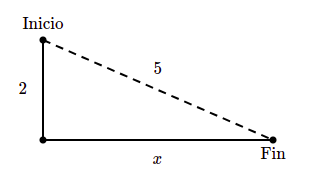
\includegraphics[width=0.4\textwidth]{../images/proverb_pitagoras_01.png}
    \end{center}
    \caption{Dibujo elaborado por Simón antes de morir.}
    \label{fig:proverb_pitagoras_01}
\end{figure}
\textbf{¿Cuántos kilómetros caminó Simón hacia el este?}\\
\textit{Redondea tu respuesta a la décima de km más cercano.}